\documentclass{article}
\usepackage{amsmath}
\usepackage{amssymb}
\usepackage{enumerate}
\usepackage{pgfplots}

\makeatletter
\renewcommand{\abstractname}{Instructions}
\makeatother

\title{MAT -- 112: Calculus I and Modeling\\
\large{EFY 3}}
\author{Thomas R. Cameron}
\date{February 5, 2018}

\begin{document}
\maketitle

\begin{abstract}
Please complete each of the following problems. You should work in groups of three, or at most four, and hand in only one submission per group. Be sure that your arguments are well justified and presented clearly. 
\end{abstract}

\paragraph*{Problem 1.}	Use the plot below to compute the average rate of change of $f$ over the intervals $[1,2]$, $[1,1.5]$, and $[1,1.25]$.
\begin{figure}[h]
\centering
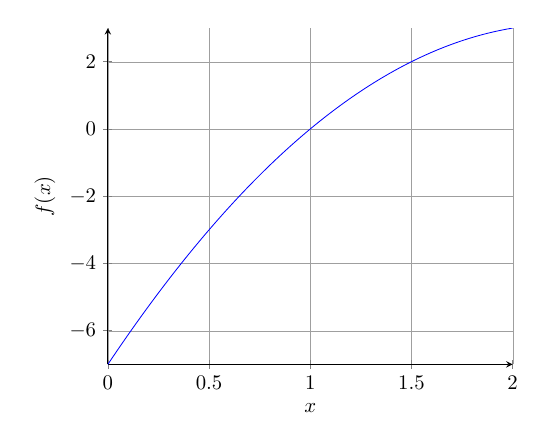
\begin{tikzpicture}[scale=0.75]
\begin{axis}[
	axis lines = left,
	xlabel = $x$,
	ylabel = $f(x)$,
	grid = both,
	grid style = {line width=0.1pt, draw=gray!75},
]
\addplot [
	domain = 0:2,
	samples = 100,
	color = blue,
]
{-7+9*x-2*x^2};
\end{axis}
\end{tikzpicture}
\end{figure}~\\
Use these average rate of change values to estimate the instantaneous rate of change of $f$ at the point $x=1$. 

\paragraph*{Solution:} The average rate of change ($ARC$) over the three intervals is given below.
\begin{itemize}
\item	Over $[1,2]$: $ARC=\frac{3-0}{2-1}=3$.
\item	Over $[1,1.5]$: $ARC=\frac{2-0}{1.5-1}=4$.
\item Over $[1,1.25]$: $ARC=\frac{1-0}{1.25-1}=4$. 
\end{itemize}
It appears that the limit is approaching $4$. This is estimate is off by $1$, the instantaneous rate of change of $f$ at $1$ is equal to $5$, but the best we can do given the data we are given. 

\paragraph*{Problem 2.}	A ball is thrown in the air with initial velocity $19.6~m/s$ and at an initial height of $0.4~m$. The height of the ball as a function of time is given by the equation
\[
h(t)=-4.9t^2+19.6t+0.4
\]
and is plotted below.
\begin{figure}[h]
\centering
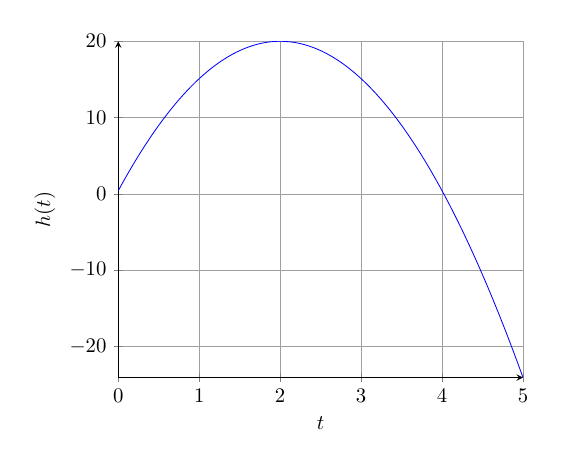
\begin{tikzpicture}[scale=0.75]
\begin{axis}[
	axis lines = left,
	xlabel = $t$,
	ylabel = $h(t)$,
	grid = both,
	grid style = {line width=0.1pt, draw=gray!75},
]
\addplot [
	domain = 0:5,
	samples = 100,
	color = blue,
]
{-4.9*x^2+19.6*x+0.4};
\end{axis}
\end{tikzpicture}
\end{figure}~\\

\begin{enumerate}[(i.)]
\item	 Use the problem description and intuition to find the instantaneous velocity at $t=0$ and $t=2$. Provide explanation.
\item	Find the time when the ball hits the ground.
\item	Find the instantaneous velocity of the ball when it hits the ground. 
\end{enumerate}

\paragraph*{Solution:}
\begin{enumerate}[(i.)]
\item	At $t=0$, the velocity must be equal to the initial velocity of $19.6~m/s$. At $t=2$, the ball has reached its peak and the instantaneous velocity is $0~m/s$. 
\item	The ball hits the ground when $h(t)=0$. We can find the possible values using the quadratic formula
\[
t=\frac{-19.6\pm\sqrt{(19.6)^2-4(-4.9)(0.4)}}{2(-4.9)}=-0.02,~4.02.
\]
We are only interested in the positive value. Thus, the ball hits the ground after $4.02~s$. 
\item	To find the instantaneous velocity of $h(t)$ at the point $a$, we must find the following limit
\[
\lim_{x\rightarrow 0}\frac{h(a+x)-h(a)}{x}.
\]
Since, we cannot simply plug-in zero, we must simplify this limit. Note that
\begin{align*}
h(a+x)-h(a)&=[-4.9(a+x)^{2}+19.6(a+x)+0.4]-[-4.9a^{2}+19.6a+0.4] \\
&=[-4.9(a^{2}+2ax+x^{2})+19.6(a+x)]-[-4.9a^{2}+19.6a] \\
&=-4.9(2ax+x^{2})+19.6x.
\end{align*}
Therefore, the instantaneous velocity of $h(t)$ at the point $a$ is given by
\begin{align*}
\lim_{x\rightarrow 0}\frac{-4.9(2ax+x^{2})+19.6x}{x}&=\lim_{x\rightarrow 0}-4.9(2a+x)+19.6 \\
&=-4.9(2a)+19.6.
\end{align*}
Plugging in $a=4.02$, we find that the instantaneous velocity of $h(t)$ at $4.02$ is equal to $-19.796~m/s$. Note that this is only slight faster than the ball's initial speed, since the ball started at a mere height of $0.4~m$. 
\end{enumerate}

\end{document}